\section{Ejercicio 3: M\'aquina de Moore}
En esta secci\'on se desea dise\~ar una m\'aquina de estados implementada con m\'quina de Moore que cumpla con la mostrada en la Figura \ref{fig:TARGET}.
\begin{figure}[H]
    \centering
    \resizebox{0.8\textwidth}{!}{
    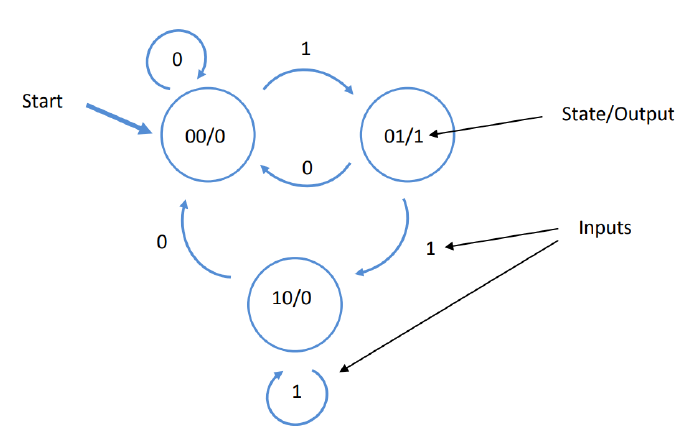
\includegraphics{../EJ3/Recursos/TARGET}
    }
    \caption{M\'aquina de estados en base a la cual se realiza el dise\~no}
    \label{fig:TARGET}
\end{figure}
Este comportamiento se corresponde con un detector de flancos que mantiene su salida en alto por un ciclo de \textit{clock}.
\subsection{Dise\~no de M\'aquina de Estados}
Se puede observar en la Tabla \ref{tab:STATE_TABLE} la tabla de estados correspondiente a la m\'aquina presentada en la Figura \ref{fig:TARGET}. Cabe aclarar que, en esta implementaci\'on se decide no fijar la salida en los estados no utilizados y utilizarlos como \textit{don't care} para facilitar el dise\~no.
\begin{table}[H]
    \centering
    \resizebox{0.4\textwidth}{!}{%
    \begin{tabular}{cccc}
    \hline
    Estado Actual & \multicolumn{2}{c}{Estado Siguiente} & Salida \\ \hline
    \multirow{2}{*}{$y_2$$y_1$} & $\omega=0$ & $\omega=1$ & \multirow{2}{*}{Z} \\
     & $Y_2$$Y_1$ & $Y_2$$Y_1$ &  \\ \hline
    00 & 00 & 01 & 0 \\
    01 & 00 & 10 & 1 \\
    10 & 00 & 10 & 0 \\
    11 & xx & xx & x \\ \hline
    \end{tabular}%
    }
    \caption{Tabla de estados de la máquina de Moore}
    \label{tab:STATE_TABLE}
\end{table}
Al haber 3 estados, es necesario utilizar 2 Flip Flops, en este caso D, para implementarla. 
Se resuelven entonces los mapas de Karnaugh para obtener el circuito que resuelve la Tabla \ref{tab:STATE_TABLE}.
\begin{figure}[H]
    \centering    
        \begin{Karnaughvuit}
        \maxterms{0,1,2,5,6}
        \minterms{4}
        \indeterminats{7, 3}
        \implicantsol{4}{red}
        \end{Karnaughvuit}
        \caption{Karnaugh para el estado siguiente $Y_1$}    
\end{figure}     
De este mapa se obtiene la soluci\'on que se muestra en \ref{eq:Y1}     
\begin{equation}
    Y_1 = \omega \cdot \overline{y_1}\cdot \overline{y_2}
    \label{eq:Y1}
\end{equation}      

\begin{figure}[H]
    \centering    
        \begin{Karnaughvuit}
        \maxterms{0,1,2,4}
        \minterms{5,6}
        \indeterminats{7, 3}

        \implicant{5}{7}{red}
        \implicant{7}{6}{blue}    

        \end{Karnaughvuit}
        \caption{Karnaugh para la variable $Y_2$}    
\end{figure}
De este mapa se obtiene la soluci\'on que se muestra en \ref{eq:Y2}  
\begin{equation}
    Y_2 = \omega \cdot y_1 + \omega \cdot y_2
    \label{eq:Y2}
\end{equation}
Adem\'as, es posible observar en la tabla de estados que $Z = y_1$. Si bien esto fija el valor de salida en el caso de que el estado actual fuera $y_2-y_1 = 1-1$, como en principio este estado no es v\'alido nunca deber\'ia suceder. Mas all\'a de esto, se define la salida como \textit{don't care} en ese caso, as\'i que tampoco presenta un problema.
Se presenta entonces, en la Figura \ref{fig:CIRCUIT}, el circuito l\'ogico obtenido a partir de resoluci\'on anterior.
\begin{figure}[H]
    \centering
    \resizebox{0.8\textwidth}{!}{
    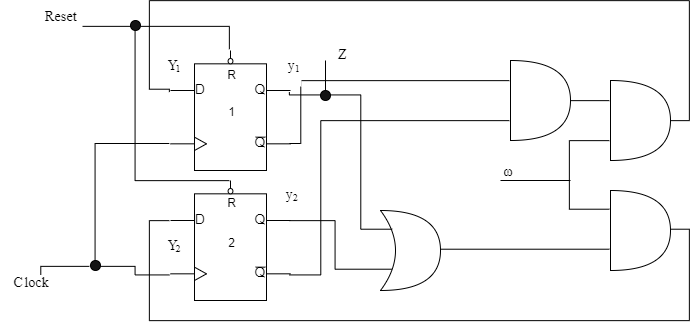
\includegraphics{../EJ3/Recursos/CIRCUIT}
    }
    \caption{Circuito implementado}
    \label{fig:LEVEL_SHIFTER}
\end{figure}
Se puede observar que se agrega una entrada adicional de reset, para poder resetear los flipflops al iniciar, comenzando en un estado v\'alido

\subsection{Level Shifters}
Si bien entradas y salidas del circuito son de 5V-0V, se dise\~na la l\'ogica interna de la m\'aquina de estados para que funcione a 3.3V. Se utilizan con este fin \textit{level shifters} en  las entradas y salidas del sistema.
Luego de contrastar el funcionamiento de las opciones disponibles que cumplen con lo requerido, se concluye que la de mejor funcionamiento en cuanto a sus caracter\'isticas, como tiempo de propagaci\'on y tiempo de rise, es presentada en la Figura \ref{fig:LEVEL_SHIFTER}.

\begin{figure}[H]
    \centering
    \resizebox{0.8\textwidth}{!}{
    \includegraphics{../EJ3/Recursos/mos_interface}
    }
    \caption{Level shifter utilizado}
    \label{fig:LEVEL_SHIFTER}
\end{figure}
\subsection{Regulador de tensi\'on}
Para obtener una tensi\'on constante en 3.3V, que se utilizan tanto  para la alimentaci\'on de los circuitos integrados, como para los \textit{level shifters}, se implementa un regulador de tensi\'on simple con un diodo zener y una resistencia.
A pesar de que el regulador funciona correctamente, se observa como un fallo en su dise\~no que la corriente que consume es muy elevada. Se asume este defecto a la baja resistencia utilizada en el regulador. 
\subsection{Mediciones y resultados}
Se puede ver en la Figura \ref{fig:GRAPH1} se puede ver como responde la m\'aquina de estados ante una entrada que se mantiene en alto por menos de un ciclo de clock, es decir, del estado 0-0 al estado 0-1 y de nuevo al estado 0-0.

\begin{figure}[H]
    \centering
    \resizebox{0.8\textwidth}{!}{
    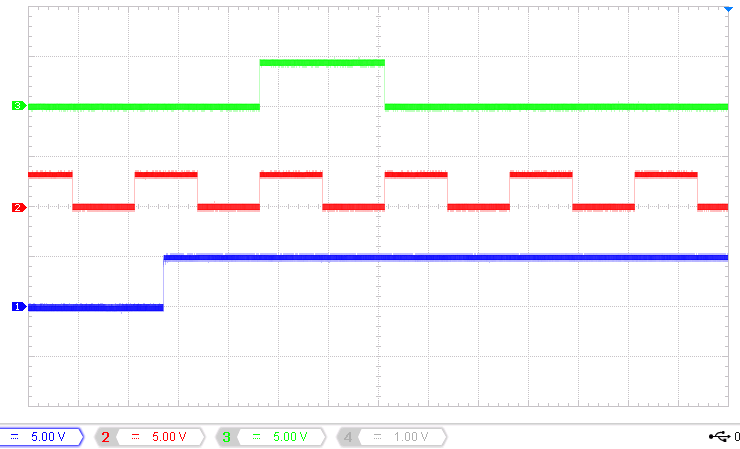
\includegraphics{../EJ3/Recursos/FOTO1}
    }
    \caption{del estado 0-0 al estado 0-1 y de nuevo al estado 0-0..Entrada en azul, clock en rojo y salida en verde}
    \label{fig:GRAPH1}
\end{figure}

En la Figura \ref{fig:GRAPH2} se observa la respuesta de la m\'aquina de estados a una entrada que se mantiene en alto por m\'as tiempo del que dura un per\'iodo del clock, es decir la transici\'on 0-0, 0-1, 1-0.
\begin{figure}[H]
    \centering
    \resizebox{0.8\textwidth}{!}{
    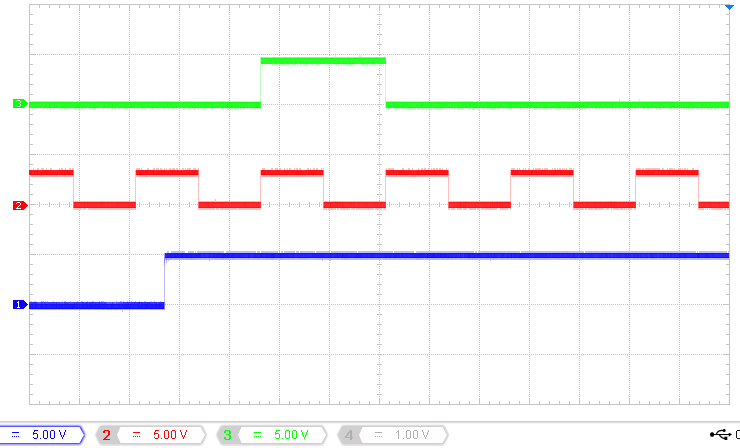
\includegraphics{../EJ3/Recursos/FOTO2}
    }
    \caption{Transici\'on 0-0, 0-1, 1-0. Entrada en azul, clock en rojo y salida en verde}
    \label{fig:GRAPH2}
\end{figure}

Se puede observar que en todos los casos el sistema responde en concordancia con lo esperado.